\RequirePackage{luatex85}
\documentclass[tikz]{standalone}
\usepackage{tikz-qtree}
\usetikzlibrary{shadows,trees}
\tikzset{
edge from parent fork down,
level distance=4cm,
every node/.style=
    {top color=white,
    bottom color=blue!25,
    rectangle,rounded corners,
    minimum height=8mm,
    draw=blue!75,
    very thick,
    drop shadow,
    align=center,
    text depth = 0pt
    },
edge from parent/.style=
    {draw=blue!50,
    thick
    }}
\begin{document}
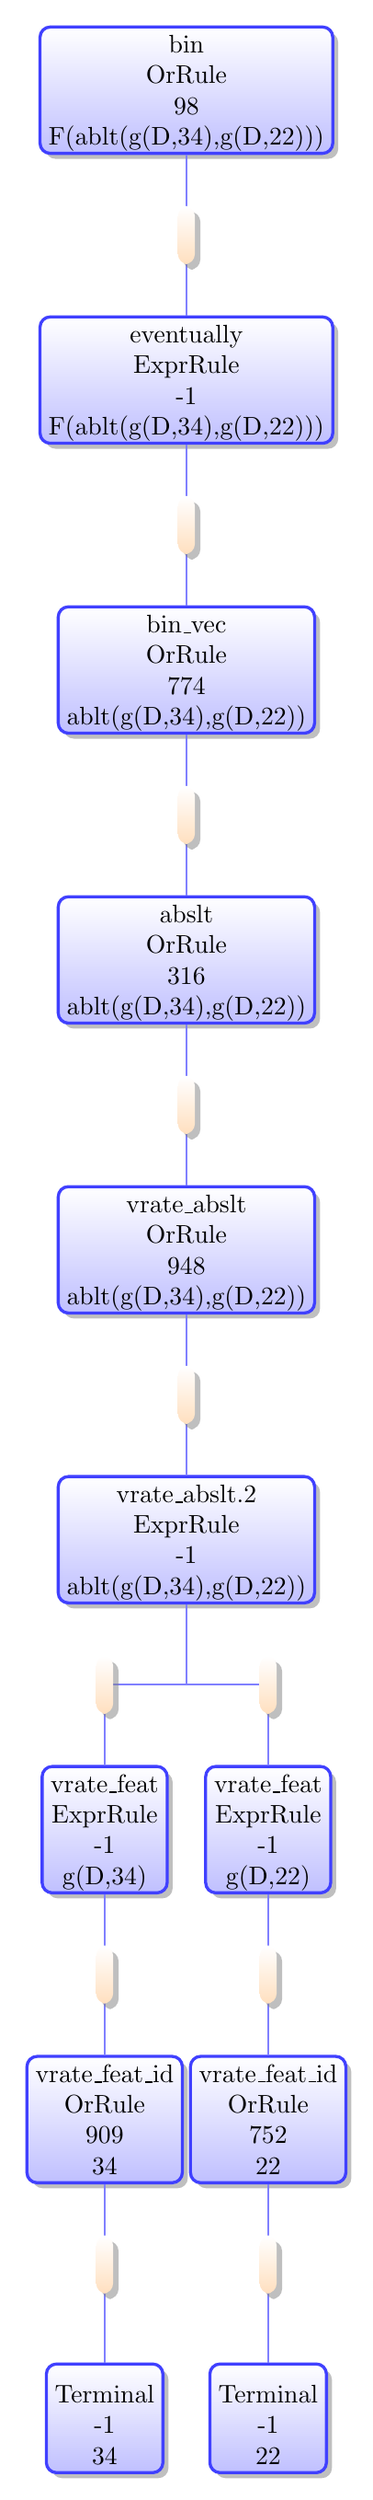
\begin{tikzpicture}[]
\Tree [.{bin\\OrRule\\98\\F(ablt(g(D,34),g(D,22)))}
\edge node[draw=none,bottom color=orange!25]{}; [.{eventually\\ExprRule\\-1\\F(ablt(g(D,34),g(D,22)))}
\edge node[draw=none,bottom color=orange!25]{}; [.{bin\_vec\\OrRule\\774\\ablt(g(D,34),g(D,22))}
\edge node[draw=none,bottom color=orange!25]{}; [.{abslt\\OrRule\\316\\ablt(g(D,34),g(D,22))}
\edge node[draw=none,bottom color=orange!25]{}; [.{vrate\_abslt\\OrRule\\948\\ablt(g(D,34),g(D,22))}
\edge node[draw=none,bottom color=orange!25]{}; [.{vrate\_abslt.2\\ExprRule\\-1\\ablt(g(D,34),g(D,22))}
\edge node[draw=none,bottom color=orange!25]{}; [.{vrate\_feat\\ExprRule\\-1\\g(D,34)}
\edge node[draw=none,bottom color=orange!25]{}; [.{vrate\_feat\_id\\OrRule\\909\\34}
\edge node[draw=none,bottom color=orange!25]{}; [.{\\Terminal\\-1\\34}
]]]\edge node[draw=none,bottom color=orange!25]{}; [.{vrate\_feat\\ExprRule\\-1\\g(D,22)}
\edge node[draw=none,bottom color=orange!25]{}; [.{vrate\_feat\_id\\OrRule\\752\\22}
\edge node[draw=none,bottom color=orange!25]{}; [.{\\Terminal\\-1\\22}
]]]]]]]]];

\end{tikzpicture}
\end{document}
